\chapter{Methods}
\section{Reproduction}
Throughout the whole paper there is a need to describe every detail and every
step in a precise manner to make sure all created results can be reproduced by
others. First and foremost this reproduction demand has to be ensured in the
"methods" chapter.

Also very important are:
\begin{itemize}
	\item A chronological order of all steps (including software versions,
	details, data-handling, ..) 
	\item What method was used to solve each part of the task?  
	\item What data versions created which results?
\end{itemize}

\begin{figure}[ht]
    \centering
    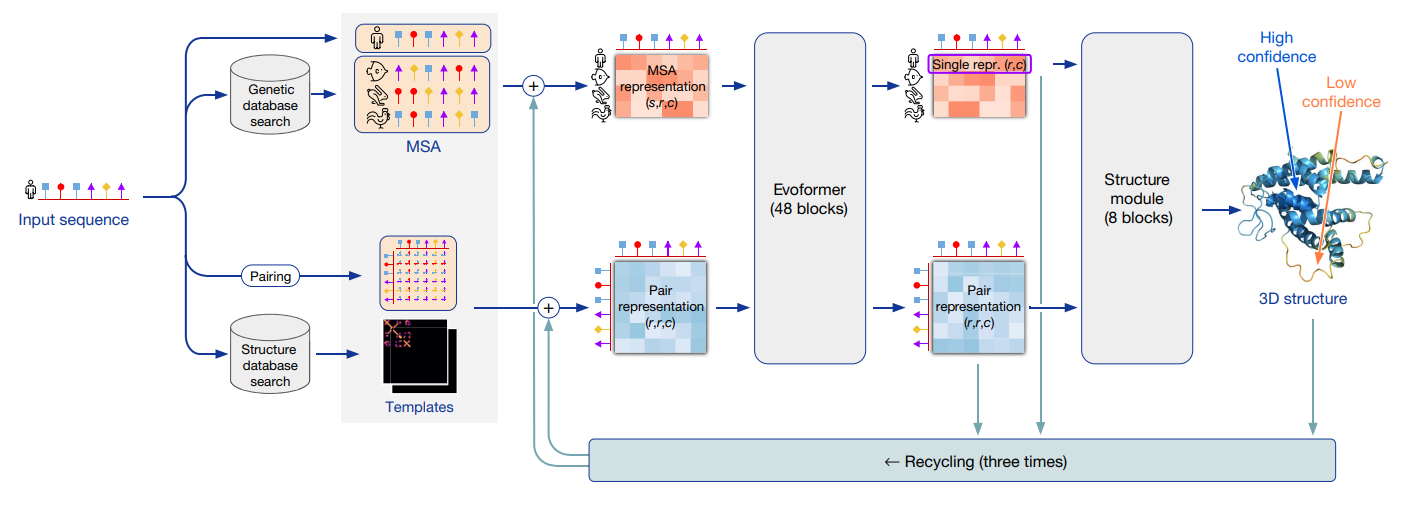
\includegraphics[width=1\textwidth]{figures/alphafold_architecture.png}
    \caption{Example of a captiones figure}
    \label{modelarch}
\end{figure}
This is a single-line code example:
\begin{verbatim}
    $ docker run --rm --gpus all nvidia/cuda:11.0-base nvidia-smi
\end{verbatim}
\section{Formula examples}
Scores below 0.2 belong to randomly selected unrelated proteins, according 
to stringent statistics of structures in the \acrshort{PDB}, while those with
more than 0.5 generally have the same protein fold (\cite{Beispiel1}) oder \parencite{Beispiel1}. The TM-score
is calculated defined by:
\[ TM-score = max 
\begin{bmatrix}
\label{complex_formula_1}
\frac{1}{L_{target}}\sum_{i}^{L_{common}} \frac{1}{1+(\frac{d_i}{d_0(L_{target})})^2}
\end{bmatrix}\]
Where L$_{target}$ is the length of the amino acid sequence of the target
protein, and L$_{common}$ is the number of residues that appear in both the
template and target structures, d$_{i}$ is the distance between the $i$th pair
of residues in the template and target structures, and $d_{0} (L_{target})$ is
a distance scale that normalizes distances and is defined by:
\[ d_{0} (L_{target}) = 1.24\sqrt[3]{L_{target}-15-1.8} \]

This is a refererence to the labeled (numbered) formula [\ref{complex_formula_1}]
When comparing two protein structures that have the same residue order, L$_{common}$ 
reads from the C-alpha order number of the structure files. The \acrshort{RMSD}
value is defined by: \[ RMSD = \sqrt{\frac{1}{N}\sum_{i=1}^{N} \delta i^2} \]
Where $\delta$i is the distance between atom i and either a reference structure 
or the mean position of the N equivalent atoms.


\begin{table}[H]
  \begin{center}
    \caption[Distribution of values tested during simulated annealing in 4th
    quartile of high scoring parameter sets]{Distribution of values tested during
    simulated annealing in 4th quartile of high scoring parameter sets (mean
    F2-Scores $>$ 0.6454).}
    \begin{tabular}{c r r r r r r r}%
      \toprule{}%
      Parameter & Minimum & 1st Quartile & Median & Mean \\
      \midrule{}%
      $\alpha$        & 0.1000 & 0.2000 & 0.4000 & 0.4692     \\
      $\beta$         & 0.0476 & 0.3704 & 0.4545 & 0.4622     \\
      $\omega$        & 0.0476 & 0.1250 & 0.2105 & 0.2324     \\
      $\sigma$        & 0.0476 & 0.1875 & 0.3077 & 0.3054     \\
      Sprot-$w$       & 10.0000 & 20.0000 & 30.0000 & 41.02009738 \\
      Sprot-$\delta$  & 0.1000 & 0.3000 & 0.5000 & 0.5365    \\
      trEMBL-$w$      & 10.0000 & 50.0000 & 70.0000 & 67.10005704 \\
      trEMBL-$\delta$ & 0.1000 & 0.5000 & 0.7000 & 0.6823     \\
      TAIR-$w$        & 10.0000 & 30.0000 & 50.0000 & 53.79005853 \\
      TAIR-$\delta$   & 0.1000 & 0.3000 & 0.5000 & 0.5392     \\
      \bottomrule{}%
    \end{tabular}
    \label{tbl:value_table}
  \end{center}
\end{table}

This is an example on how to reference a table that has the
\verb|\label{tbl:value_table}| by using \verb|\ref{tbl:value_table}|: The
estimated values are listed in table \ref{tbl:value_table}.
